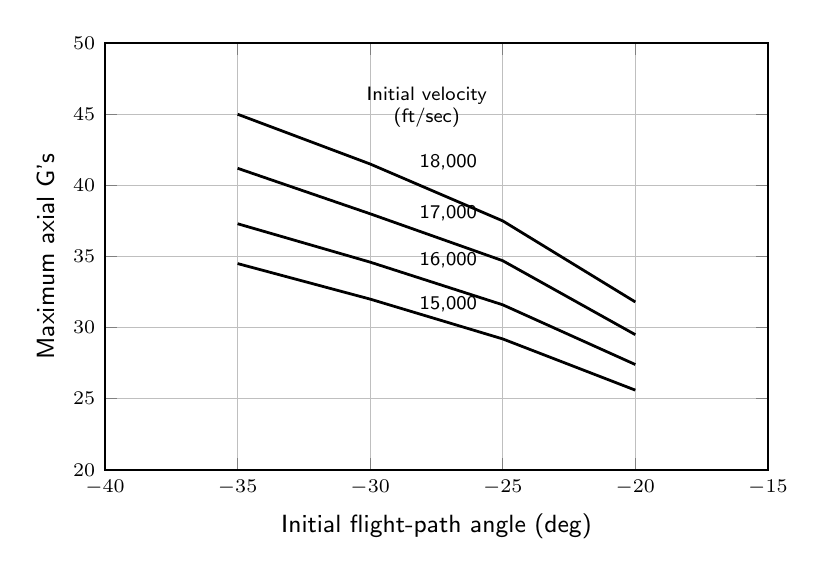
\begin{tikzpicture}
\begin{axis}[
  width=10.0cm,height=7.0cm,
  xmin=-40,xmax=-15,ymin=20,ymax=50,
  xtick={-40,-35,-30,-25,-20,-15},
  ytick={20,25,30,35,40,45,50},
  grid=major,
  axis line style={line width=0.8pt},
  tick label style={font=\scriptsize},
  label style={font=\sffamily\small},
  xlabel={Initial flight-path angle (deg)},
  ylabel={Maximum axial G's},
  ylabel style={align=center},
]
  \addplot[line width=1.0pt] coordinates {(-35,34.5) (-30,32.0) (-25,29.2) (-20,25.6)};
  \addplot[line width=1.0pt] coordinates {(-35,37.3) (-30,34.6) (-25,31.6) (-20,27.4)};
  \addplot[line width=1.0pt] coordinates {(-35,41.2) (-30,38.0) (-25,34.7) (-20,29.5)};
  \addplot[line width=1.0pt] coordinates {(-35,45.0) (-30,41.5) (-25,37.5) (-20,31.8)};
  \node[font=\sffamily\scriptsize,align=center,anchor=west] at (axis cs:-30.5,45.5) {Initial velocity\\(ft/sec)};
  \node[font=\sffamily\scriptsize,anchor=west] at (axis cs:-28.5,41.6) {18,000};
  \node[font=\sffamily\scriptsize,anchor=west] at (axis cs:-28.5,38.0) {17,000};
  \node[font=\sffamily\scriptsize,anchor=west] at (axis cs:-28.5,34.7) {16,000};
  \node[font=\sffamily\scriptsize,anchor=west] at (axis cs:-28.5,31.6) {15,000};
\end{axis}
\end{tikzpicture}
